\documentclass[german, a4paper, 12pt]{scrartcl}

\usepackage[no-math]{fontspec}
\defaultfontfeatures{Ligatures=TeX}
\usepackage{polyglossia}
\setdefaultlanguage{german}

\usepackage{wrapfig}
\begin{document}
\begin{wrapfigure}[]{r}{0cm}
	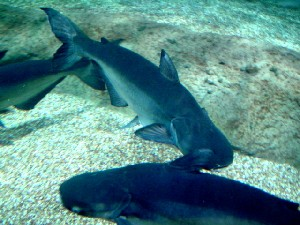
\includegraphics[width=7cm]{wels.jpg}
	\caption{Ein Wels.}
\end{wrapfigure}
\noindent Der Mekong-Riesenwels (Pangasianodon gigas) ist die größte Art der Familie der Haiwelse (Pangasiidae) und einer der größten Süßwasserfische der Welt. Er kommt ausschließlich im Mekong vor und gilt durch Überfischung und Verlust des Lebensraums als vom Aussterben bedroht. In Südostasien wird er als Flaggschiffart eingesetzt, um die Notwendigkeit des Schutzes großer Fische im Mekong zu vermitteln. Mekong-Riesenwelse zeichnen sich durch eine sehr hohe Wuchsrate aus und werden daher auch in Aquakulturprogrammen gezogen; inwieweit künstliche Nachzuchten sich zur Stützung der Wildbestände eignen, ist aber bislang unklar.

Mekong-Riesenwelse sind wie alle Haiwelse schuppenlos und haben einen langgestreckten, seitlich abgeflachten Körper. Ausgewachsene Tiere sind sehr kräftig gebaut und können eine Körperlänge von bis zu drei Metern und ein Gewicht von über 300 kg erreichen. Die Weibchen werden dabei länger und schwerer als die Männchen.
\end{document}